% !TeX spellcheck = pl_PL
\chapter{Realizacja instrumentu muzycznego}
Implementacja tworzonego syntezatora muzycznego realizowana jest na wspomnianej we wstępie płycie PADK, która opiera swoje działanie na procesorze DSP. W ramach tego implementowane jest wiele mechanizmów, które są konieczne do kompletnego działania projektu: przetwarzanie sygnałów z klawiatury muzycznej, wydobycie dźwięku z płyty PADK oraz komunikacja z interfejsem użytkownika. W niniejszym rozdziale przedstawiono podejście do realizacji wymienionych zadań. Implementacja poszczególnych algorytmów syntezy dźwięku przedstawiona zostanie w kolejnych rozdziałach.

Cały kod programu na procesor DSP napisany został w języku C. Program pisano w środowisku Code Composer Studio v6, które jest dedykowane do procesorów firmy Texas Instruments. Wgrywanie kodu na płytę odbywało się poprzez użycie debuggera XDS510 firmy Spectrum Digital. Debugger połączony jest z płytą PADK przez taśmę, a następnie przejściówkę 8-pinową.

% zdjęcie PADK z debuggerem

\section{Układ instrumentu}
% Zdjęcie i opis co z czym łączymy

\section{Płyta PADK}

\subsection{Procesor TMS320C6727}
%https://www.ti.com/lit/ds/symlink/tms320c6727.pdf?ts=1595978326019&ref_url=https%253A%252F%252Fwww.google.com%252F 
%--> glowne feature'y
%--> strona 13 wypisane w myslnikach np busy

\subsection{Peryferia komunikacyjne}

\subsection{Przetworniki DAC}



\section{Mechanizmy szybkiego przetwarzania danych}
Procesor sygnałowy TMS320C6727 jest przeznaczony między innymi do szybkiego przetwarzania danych i sygnałów. Poza wysoką szybkością taktowania procesora, firma Texas Instruments zawiera dodatkowe mechanizmy akceleracji przepływu danych i sygnałów. Zostały one opisane w poniższych podpunktach.

\subsection{McASP}
% https://www.ti.com/lit/an/sprack0/sprack0.pdf?ts=1595842361762&ref_url=https%253A%252F%252Fwww.google.com%252F
McASP to akronim od Multichannel Audio Serial Port. Jest to komunikacyjne urządzenie peryferyjne dedykowane do przetwarzania danych audio lub wideo. Został zaprojektowany w celu przypadków wymagających wielokanałowego przetwarzania dźwięku. Jedną z najbardziej przydatnych właściwości narzędzia McASP jest schemat wielozegarowy. Pozwala on na niezależność pomiędzy portami odbierającymi i nadającymi. Komunikacja, którą zarządza McASP może odbywać się poprzez interfejs I2S (ang. Inter-IC Sound), I2C (ang. Inter-Integrated Circuit) lub SPI (ang. Serial Peripheral Interface).

Kiedy dane przepływają przez McASP, mogą zostać dostosowane tak, aby reprezentacja stałoprzecinkowa używana przez kod aplikacji była niezależna od reprezentacji używanej przez urządzenia zewnętrzne, bez wymagania dodatkowej konwersji przez procesor.

W niniejszej pracy narzędzie McASP stosowane jest do przepływu danych między DAC a procesorem. W ramach inicjalizacji McASP ustawia odpowiednią szybkość próbkowania dla modułu DAC.

\subsection{dMAX}
%https://www.ti.com/lit/ug/spru795d/spru795d.pdf?ts=1595843361787&ref_url=https%253A%252F%252Fwww.google.com%252F, strona 14, Overview
Kontroler dMAX (Dual Data Movement Accelerator) obsługuje transfery zaprogramowane przez użytkownika pomiędzy kontrolerem pamięci wewnętrznej i urządzeniami peryferialnymi na procesorach DSP firmy TI. Mechanizm ten jest dedykowany szczególnie dla procesorów z serii C672x.

Zasada działania dMAX opiera się na sygnałach zdarzeń (ang. event signals). Zdarzenie zdefiniowane jest jako zmiana wartości logicznej odpowiadającego sygnału zdarzeń w rejestrze flag zdarzeń. Zdarzenie może być używane jako: wzbudzenie rozpoczęcia transferu danych lub spowodowanie wystąpienia przerwania dla CPU. Wszystkie zdarzenia posortowane są w dwie grupy: grupa niskiego priorytetu oraz grupa wysokiego priorytetu. Mechanizm dMAX może równolegle przetwarzać dwa żądania zdarzeń z każdej z grupy.

Częścią mechanizmu dMAX jest również bufor cyrkulacyjny FIFO. Pozwala on na równoczesny, asynchroniczny odczyt i zapis danych do jednego bufora dwustronnego. Narzędzie dMAX wykrywa kiedy dane zostają zapisane do bufora i natychmiastowo wywołuje odwrócenie go. Po odwróceniu, zapisane chwilę wcześniej dane mogą zostać odczytane z drugiej strony bufora, natomiast równocześnie kolejne dane zapisywane są po pierwszej stronie.


\section{Komunikacja z płytą PADK}
Do płyty PADK dołączone zostały dodatkowe biblioteki firmy Lyrtech, które ułatwiają obsługę komunikacji z płytą. Przykładem interfejsów, do których zostały utworzone nadmienione biblioteki to UART oraz MIDI.

\subsection{Komunikacja z klawiaturą muzyczną  (MIDI)}
% Datasheet "Professional Audio Development Kit Technical Reference Guide 1.4", September 2007
Jednym z podstawowych peryferiów klawiatury muzycznej jest wyprowadzenie interfejsu MIDI. Przeważnie jest to pięciopinowe gniazdo DIN. W płycie PADK zastosowano jednak dziewięciopinowe gniazdo typu D-sub. Zatem wymagało to stworzenia odpowiedniego kabla, aby połączyć klawiaturę muzyczną z płytą PADK.
Do obsługi interfejsu MIDI wykorzystana została biblioteka PADK\_MIDI.c, która zawiera takie funkcje jak:
\begin{itemize}
	\item MIDI\_Init - inicjalizacja interfejsu MIDI,
	\item MIDI\_EnableLed1, MIDI\_EnableLed2 - sterowanie diodami LED interfejsu MIDI,
	\item MIDI\_Read - odczyt przychodzących bajtów. 
\end{itemize}
Aby w jak najmniejszym stopniu obciążać procesor, obsluga interfejsu MIDI została sprowadzona jedynie do odczytywania przychodzących bajtów poprzez przerwania sprzętowe.
Jako że ramki MIDI składają się z trzech bajtów, odczytywać oraz interpretować należy kolejne 3 przychodzące bajty.
Można to osiągnąć poprzez umieszczenie funkcji MIDI\_Read z parametrem 3 (odczyt 3 bajtów za jednym razem) w obsłudze przerwania. Jednak sytuację nieco komplikuje zegar MIDI, który powoduje, że DSP będzie odczytywał regularnie bajt o wartości 0xF8. Powoduje to, że w odczytanej sekwencji 3 bajtów pojawiała się niepożądana wartość 0xF8.
\begin{figure}[H]
	\centering
	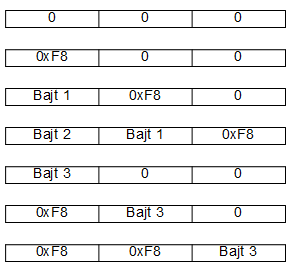
\includegraphics[width=8cm]{./grafiki/real_nofifo}
	\captionsetup{justification=centering}
	\caption{Odczytywane ramki MIDI przy braku odpowiedniej procedury odczytu.}
	\label{rys:real_nofifo}
\end{figure} 
Problem ten został zobrazowany na rysunku \ref{rys:real_nofifo}. Przedstawia on zawartość bufora wejściowego w czasie biegnącym od góry do dołu rysunku. W pokazanej sytuacji pomiędzy wywołaniem funkcji MIDI\_Read z parametrem 3, a nadejściem 3-bajtowej ramki danych, został odczytany bajt zegarowy. Ostatecznie odczytana zostanie ramka 4. oraz 7. od góry.  Oznacza to, że bajty, które miały zostać odczytane jako jedna ramka, mogą być dowolnie rozbite pomiędzy dwie obsługi przerwania. 
Aby rozwiązać ten problem, funkcja osbługi przerwania wywołuje funkcję MIDI\_Read z parametrem 1. W rezultacie kżdy przychodzący bajt wywołuje przerwanie. W obsłudze przerwania sprawdzana jest wartość bajta, jesli jest ona różna od 0xF8 (zegar MIDI), to zostaje ona dodana do trzyelementowej kolejki FIFO. W momencie gdy kolejka FIFO się zapełnia, ramka jest identyfikowana i interpretowana, a kolejka czyszczona. Działanie takiej kolejki zobrazowane jest na rysunku \ref{rys:real_fifo}.
\begin{figure}[H]
	\centering
	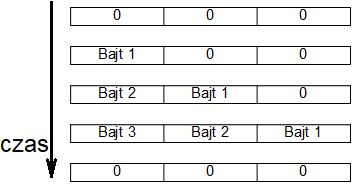
\includegraphics[width=8cm]{./grafiki/real_fifo}
	\captionsetup{justification=centering}
	\caption{Odczytywane ramki MIDI przy wykorzystaniu kolejki FIFO.}
	\label{rys:real_fifo}
\end{figure} 
Dzięki sprawdzaniu każdego przychodzącego bajta w obsłudze przerwania, do kolejki FIFO dostają się tylko istotne bajty. Dyskryminowanie wartości 0xF8 nie powinno mieć skutków ubocznych, gdyż wartość ta nie pojawia się w żadnym z bajtów ramki MIDI, poza bajtem statusu komunikatu zegarowego.
\subsection{Komunikacja z interfejsem użytkownika (UART)}
Do komunikacji z interfejsem użytkownika działajacym na komputerze klasy PC wykorzystany został interfejs RS-232, który znajduje się na płycie PADK. Do komunikacji z komputerem użyto przejściówki z RS-232 na USB. 
Do obsługi interfejsu szeregowego wykorzystana została biblioteka PADK\_UART.c, która zawiera takie funkcje jak:
\begin{itemize}
	\item UART\_Init - inicjalizacja interfejsu UART,
	\item UART\_EnableLed1, UART\_EnableLed2 - sterowanie diodami LED interfejsu UART,
	\item UART\_Read - odczyt przychodzących bajtów,
	\item UART\_Write - nadanie bajtów.
\end{itemize}
Aby zapewnić wygodny w użyciu oraz odporny na błędy przepływ informacji, utworzono własny protokół.
\begin{figure}[H]
	\centering
	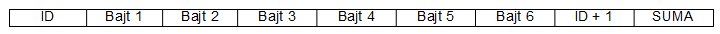
\includegraphics[width=16cm]{./grafiki/real_uartframe}
	\captionsetup{justification=centering}
	\caption{Struktura ramki protokołu.}
	\label{rys:real_uartframe}
\end{figure}
Na rysunku \ref{rys:real_uartframe} pokazana została struktura 9-bajtowej ramki danych, która jest przesyłana między DSP a komputerem. Składa się ona z dwóch bajtów identyfikujących, sześciu bajtow danych oraz jednego bajta sumy kontrolnej. Podobnie jak w przypadku MIDI, do identyfikacji i interpretacji przychodzących ramek, wykorzystywana jest kolejka FIFO. Tym razem ma ona rozmiar 9 bajtów. Bajty przychodzące są odczytywane pojedynczo przy wykorzystaniu przerwania sprzetowego i wpisywane do kolejki FIFO. W momencie gdy na pierwszym miejscu w kolejce znajdzie się odpowiedni bajt identyfikujący ramkę, a na miejscu ósmym znajdzie się wartość tego bajta powiększona o jeden, to jest domniemanie, że odebrana została jakaś ramka danych. W ramach upewnienia się, dodatkowo obliczana jest suma kontrolna z bajtów danych. Gdy ramka przejdzie taką weryfikację, zostaje następnie przetworzona w zależności od informacji, które niesie. Opisany mechanizm działa zarówno na procesorze DSP, jak i na komputerze PC.
Takie dziewięciobajtowe ramki pozwalają na przesyłanie na przykład całych zmiennych 4-bajtowych lub jednocześnie trzech liczb 2-bajtowych. 
\section{Wydobycie dźwięku (DAC)}
% pamiętać o: odniesienie do dMAX z buforem cyrkulacyjnym



\section{Klawiatura polifoniczna}




\section{Wykorzystanie algorytmu FFT}
%http://www.secs.oakland.edu/~ganesan/old/courses/CSE671SU08/CSE%20671%20Lab%204%20ANC%20Code/Lee's%20adaptive%20wiener%20filter/DSPF_sp_cfftr2_dit.h

%https://processors.wiki.ti.com/index.php/C674x_DSPLIB <--- funkcje dsp_lib

W pamięci ROM procesorów z serii TMS320C672x zostały umieszczone specjalnie zoptymalizowane biblioteki, dedykowane do szybkiego przetwarzania sygnałów cyfrowych. Skompilowane biblioteki zostały napisane w asemblerze w celu większej efektywności obliczeniowej. 

%https://www.ti.com/lit/an/spraas8/spraas8.pdf?ts=1596035199216&ref_url=https%253A%252F%252Fwww.google.com%252F
W naszym projekcie, użyta została biblioteka \emph{DSP Library} z procesora TMS320C6727, która posiada efektywne obliczeniowo funkcje takie jak: transformacja FFT, odwracanie macierzy lub operacja na wektorach. W celu zawarcia jej w projekcie z programem na DSP, należało zmodyfikować komende pliku linkera dodając do niej bibliotekę o nazwie \emph{c67xdsplibR.lib}. Dodatkowo zmieniono sekcje pamięci, tak aby linker został odpowiednio poinstruowany, do których obszarów pamięci powinien się odnieść. Do pełnej transformacji FFT użyto dwóch funkcji z nadmienionej biblioteki: DSPF\_sp\_cfftr2\_dit() oraz DSPF\_sp\_bitrev\_cplx(). 

%http://software-dl.ti.com/jacinto7/esd/processor-sdk-rtos-jacinto7/latest/exports/docs/dsplib_c66x_3_4_0_0/docs/doxygen/html/dsplib_html/group___f_f_t.html
Funkcja DSPF\_sp\_cfftr2\_dit() odpowiada za przeprowadzenie algorytmu FFT radix-2 dla liczb zmiennoprzecinkowych. Sygnał na wejściu powinien posiadać N liczb zespolonych ułożonych w tablicy kolejno w pary liczb rzeczywistych i urojonych. Jako drugi argument wejściowy funkcja przyjmuje tablicę współczynników obrotu dla FFT o długości N/2. Współczynniki obrotu utworzone zostają przez zestaw trzech funkcji udostępnionych na stronie producenta procesora. %https://www.rose-hulman.edu/class/ee/yoder/ece581/TI%20library/C6700/dsplib/support/fft/tw_r2fft.c <-- twiddle factors
Opisywana funkcja może również zostać użyta do uzyskania transformaty odwrotnej poprzez zmianę kolejności współczynników obrotu, a na końcu podzielenie wynikowej transformaty przez N, czyli według wzoru \ref{equ:idft_upr}.

%http://software-dl.ti.com/jacinto7/esd/processor-sdk-rtos-jacinto7/latest/exports/docs/dsplib_c66x_3_4_0_0/docs/doxygen/html/dsplib_html/group___d_s_p_f__sp__bitrev__cplx.html
Funkcja DSPF\_sp\_bitrev\_cplx() odpowiada za zamianę kolejności próbek w tablicy wynikowej otrzymanej z funkcji realizującej algorytm FFT. Zmiana kolejności elementów tablicy realizowana jest przez odczytanie indeksów tablicy jako liczb w postaci bitowej, a następnie dokonanie lustrzanego odbicia każdego indeksu z osobna (ang. bit-reverse).


\section{Generowanie przebiegów czasowych}
% waveformy wykorzystywane w subtractive, additive oraz FM - dlatego opisywane tutaj


\section{ADSR}



\section{Interfejs użytkownika}